\documentclass[A4]{article1}

\def\vol{00}
\def\issue{000}
\def\copyrightyear{2050}

\usepackage{natbib}
\usepackage[justification=justified]{caption}
\usepackage{booktabs}
\usepackage{placeins}
\usepackage{xcolor}
%\usepackage{pdflscape}
\usepackage{rotating}
\usepackage{xr}
%\externaldocument{bppGDI-SI}

%\bibpunct{[}{]}{,}{n}{}{;}

%\usepackage[switch, modulo]{lineno}
%\linenumbers

\allowdisplaybreaks[2]

\DeclareMathOperator{\E}{\mathbb{E}}
\DeclareMathOperator{\V}{\mathbb{V}}
\newcommand{\U}{\mathbb{U}}
\renewcommand{\P}{\mathbb{P}}
\renewcommand{\d}{\mathrm{d}}
\DeclareMathOperator{\e}{\mathrm{e}}

\newcommand{\red}[1]{{\color{red}{#1}}}
\newcommand{\blue}[1]{{\color{blue}{#1}}}
\newcommand{\pink}[1]{{\color{magenta}{#1}}}
\newcommand{\purple}[1]{{\color{purple}{#1}}}

\begin{document}

\title[Heuristic species delimitation] {HMDelimit: A pipeline for heuristic species delimitation
   under the multispecies coalescent model using multilocus sequence data}

\author[
	Kornai \textit{et~al.}]{Daniel Kornai (orcid: 0000-0003-4919-2384)\,$^{1}$, 
	Tom\'{a}\v{s} Flouri (orcid: 0000-0002-8474-9507)\,$^{1}$, and
	Ziheng Yang (orcid: 0000-0003-3351-7981)\,$^{1,}$\footnote{to whom correspondence should be addressed}}

\address{
	$^1$Department of Genetics, Evolution and Environment, University College London, UK \\
}

\date{Received on xxxx, revised on xxxx, accepted on xxxx}


\begin{abstract}
The multispecies coalescent (MSC) model accommodates genealogical variations across
the genome and provides a natural framework for comparative analysis of genomic
sequence data to infer the history of species divergence and gene flow.  Given a set
of populations, hypotheses of species delimitation (and species phylogeny) may be
formulated as instances of MSC models (e.g., MSC for one species versus MSC for two
species) and compared using Bayesian model selection. This approach, implemented in
the Bayesian program \textsc{bpp}, has been found to be prone to over-splitting.
Alternatively heuristic criteria based on population parameters under the MSC model
(such as population/species divergence times, population sizes, and migration rates)
estimated from genomic sequence data may be used to delimit species.  Here we extend
the approaches of \cite{Jackson2017} and \cite{Leache2019} based on the genealogical
divergence index (\textit{gdi}) and develop hierarchical merge and split algorithms
for species delimitation, and implemented them as a python pipeline.  Applied to
data simulated under a model of isolation by distance, the approach was able to
recover the correct species delimitation, whereas model comparison by \textsc{bpp}
failed.  Analyses of empirical datasets suggested that the procedure may avoid the
problem of over-splitting.  We discuss possible strategies for accommodating gene
flow in the procedure, as well as the challenges of species delimitation based on
heuristic criteria. \\ %
\textsc{bpp} $|$ genealogical divergence index $|$ multispecies coalescent $|$
species delimitation
\end{abstract}

\maketitle


\section{Introduction}

Accurate delimitation of species boundaries is important to characterizing patterns of
biological diversity, especially during the current global changes in climate and
environment.  Traditionally, species have been identified and distinguished using
morphological characteristics.  Molecular genetic data can provide additional
information about many processes related to species delimitation and identification,
including population identities, interspecific hybridization and gene flow, and
phylogenetic relationships among the populations and their divergence times
\citep{Jiao2021MSC}.

Given a set of populations, different species delimitations correspond to different ways
of merging populations into the same species.  Each species delimitation, combined with
the phylogeny for the delimited species, can be formulated as an instance of the
multispecies coalescent (MSC) model \citep{Rannala2003} and fitted to genomic sequence
data sampled from the modern species or populations.  Competing models can then be
compared via Bayesian model selection (i.e., using posterior model probabilities or
Bayes factors) to find the best supported delimitation.  In the Bayesian program
\textsc{bpp}, this is accomplished by using a Markov chain Monte Carlo (MCMC) algorithm
to estimate the posterior probabilities for different MSC models \citep{Yang2010,
   Yang2014, Yang2015, Flouri2018}. In simulations, \textsc{bpp} showed lower rates of
species overestimation and underestimation than the generalized mixed Yule-coalescent or
Poisson tree processes \citep{Luo2018}.  In empirical datasets, \textsc{bpp} was
effective in identifying cryptic species in many ancient lineages that were not
recognised by other molecular or morphological approaches.  For example,
\cite{Ramirez-Reyes2020} identified 13 new species of leaf-toed geckoes in a lineage
that diverged 30 Ma.

However, \textsc{bpp} has been noted to often over-split, identifying more lineages as
distinct species than many other methods \citep{Sukumaran2017}.  For example,
\cite{Campillo2020} analyzed 99 population pairs in the genus \textit{Drosophila} and
found that \textsc{bpp} identified 80 pairs as distinct species, whereas reproductive
isolation was identified in only 69 pairs.  Similarly, \citet{Bamberger2022} examined 48
\textit{Albinaria cretensis} land snail populations, and found that morphological
delimitation ?? suggested 3--9 species, \textsc{admixture} ?? suggested 15, while
\textsc{bpp} suggested 45-48. \citet{Barley2018} simulated multiple populations from a
single species that exhibits isolation by distance, and found that \textsc{bpp} delimits
geographically separated populations as distinct species. Those results suggest that the
lineages identified by \textsc{bpp} sometimes correspond to populations rather than
species \citep{Chambers2020}. Multiple studies using \textsc{bpp} have suggested
significant taxonomic reassignments not supported using other methods (e.g.,
\citealp{Wu2018} in Yunnan Bananas).  A number of authors have expressed concerns about
the apparent over-splitting of \textsc{bpp} \citep{MacGuigan2021}.

Rather than treating species delimitation as a model-selection problem, an alternative
approach is to estimate population parameters, such as population split time ($\tau$),
population sizes ($\theta$), and migration rates ($M$), and define species status using
empirical criteria based on those parameters.  For example, the `$10\times$ rule'
specifies the interspecific divergence to be at least 10 times as large as the
intraspecific diversity \citep{Hebert2004}.  

\citet{Jackson2017} suggested a criterion called the \textit{genealogical divergence
   index} (\textit{gdi}), defined using population parameters.  Consider two sequences
($a_1$ and $a_2$) sampled population $A$ and one sequence ($b$) from $B$ (see
fig.~\ref{fig:gdi-trees}).  Let the probability that the two sequences from population $A$
coalesce first, so that the gene tree is $G_1 = ((a_1, a_2), b)$, be $P_1 = \P(G_1)$. 
In the case of no gene flow, this is given as
\begin{equation} \label{eq:PG1_M0}
   P_1 = 1 - \tfrac{2}{3} \e^{-2 \tau_{AB} / \theta_A},
\end{equation} 
This is a simple function of $2\tau_{AB}/\theta_A = T_{AB}/(2N_A)$, the population
divergence time in coalescent units (with one coalescent time unit to be $2N_A$
generations in population $A$).  \citet{Jackson2017} rescaled $P_1$ so that the
\textit{gdi} ranges from 0 to 1.
\begin{equation} \label{eq:gdi}
    gdi = 1 - \e^{-2\tau_{AB} / \theta_A} = 1 - \e^{-T_{AB} / (2N_A)}.
\end{equation} 
Thus the \textit{gdi} is the probability that the two $A$ sequences coalesce before
reaching species divergence ($\tau_{AB}$) when we trace the genealogy of the sample
backwards in time. A \textit{gdi} close to 1 indicates a high level of population
divergence.  Based on a meta-analysis of data from \citet{Pinho2010}, \citet{Jackson2017}
suggest that populations are likely to be a single species if \textit{gdi} $< 0.2$, and
separate species if \textit{gdi} $> 0.7$. Intermediate values ($0.2 < $ \textit{gdi} $ <
0.7$) indicate ambiguous species status.

When there is migration between the two populations, the probability for the gene tree
$G_1$ depends on the parameters of the MSC-M model:
\begin{equation} \label{eq:PG1}
    P_1 = \P(G_1 \bigl| \tau_{AB}, \theta_A, \theta_B, \theta_{AB}, M_{AB}, M_{BA}). 
\end{equation} 
Thus the minimum and maximum of $P_1$ used by \citet{Jackson2017} for rescaling $P_1$
depend on the model parameters.  Instead, here we redefine \textit{gdi} as the
probability that the first coalescence is between the two $A$ sequences and it occurs
before reaching species divergence when we trace the genealogy backwards in time.  This
definition applies whether or not there is gene flow in the model (fig.~\ref{fig:gdi-trees}),
with $0 \le gdi \le 1$.

\citet{Leache2019} described a hierarchical merge algorithm for species delimitation
based on \textit{gdi}.  Given a set of populations and a guide tree for them, the
procedure attempts to merge two populations into one species, judged by \textit{gdi}.
Here we develop a python pipeline to automate the procedure.  We include a hierarchical
split algorithm as well.  We first describe the computation of \textit{gdi} when there
is gene flow in the model, following \citet{Leache2019}.  Then we discuss our new
pipeline.  We apply the pipeline to four empirical datasets, for giraffes, snails,
milksnakes, and sunfish.

\begin{figure} [t]
   \centering %
   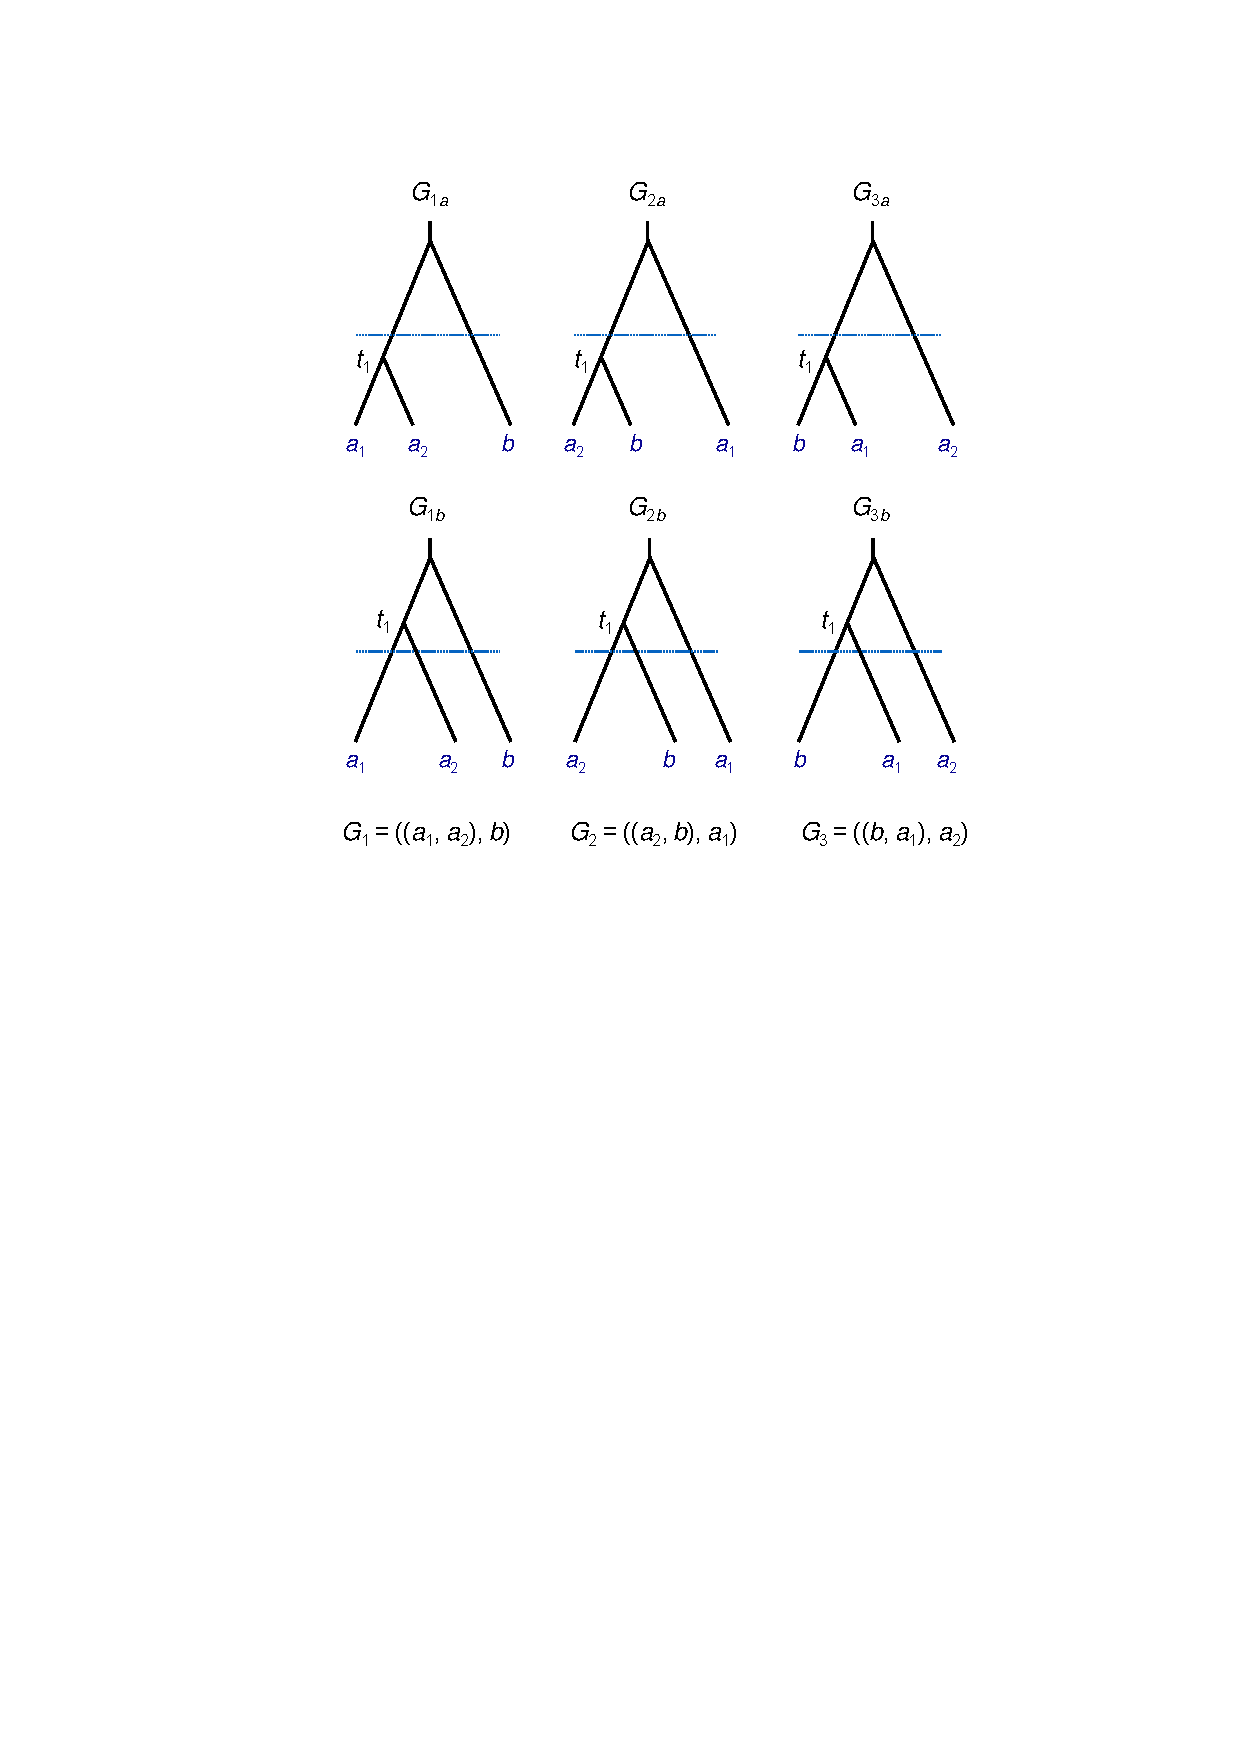
\includegraphics[scale=0.6]{figs/fig-gdi-trees} %
   
   \caption{For a locus with two sequences $a_1$, $a_2$ from species $A$ and one
      sequence $b$ from $B$, there are three possible gene trees: $G_1 = ((a_1, a_2), b)$;
      $G_2 = ((a_2, b), a_1)$; and $G_3 = ((b, a_2), a_1)$.  If the first coalescence time
      is more recent than the species divergence time (indicated by the dashed line), we
      label the gene tree as $G_{1a}, G_{2a}, G_{3a}$; otherwise they are labeled $G_{1b},
      G_{2b}, G_{3b}$.  We have $gdi = \P(G_{1a})$.  The \textit{gdi} is the probability
      that two $A$ sequences coalesce first and before the population split.  Note that if
      there is no gene flow between species $A$ and $B$, gene trees $G_{2b}$ and $G_{3b}$
      are impossible.  %
   } \label{fig:gdi-trees}
\end{figure}


\section{Computation of gdi under the MSC-M model}

\begin{figure} [t]
   \centering %
   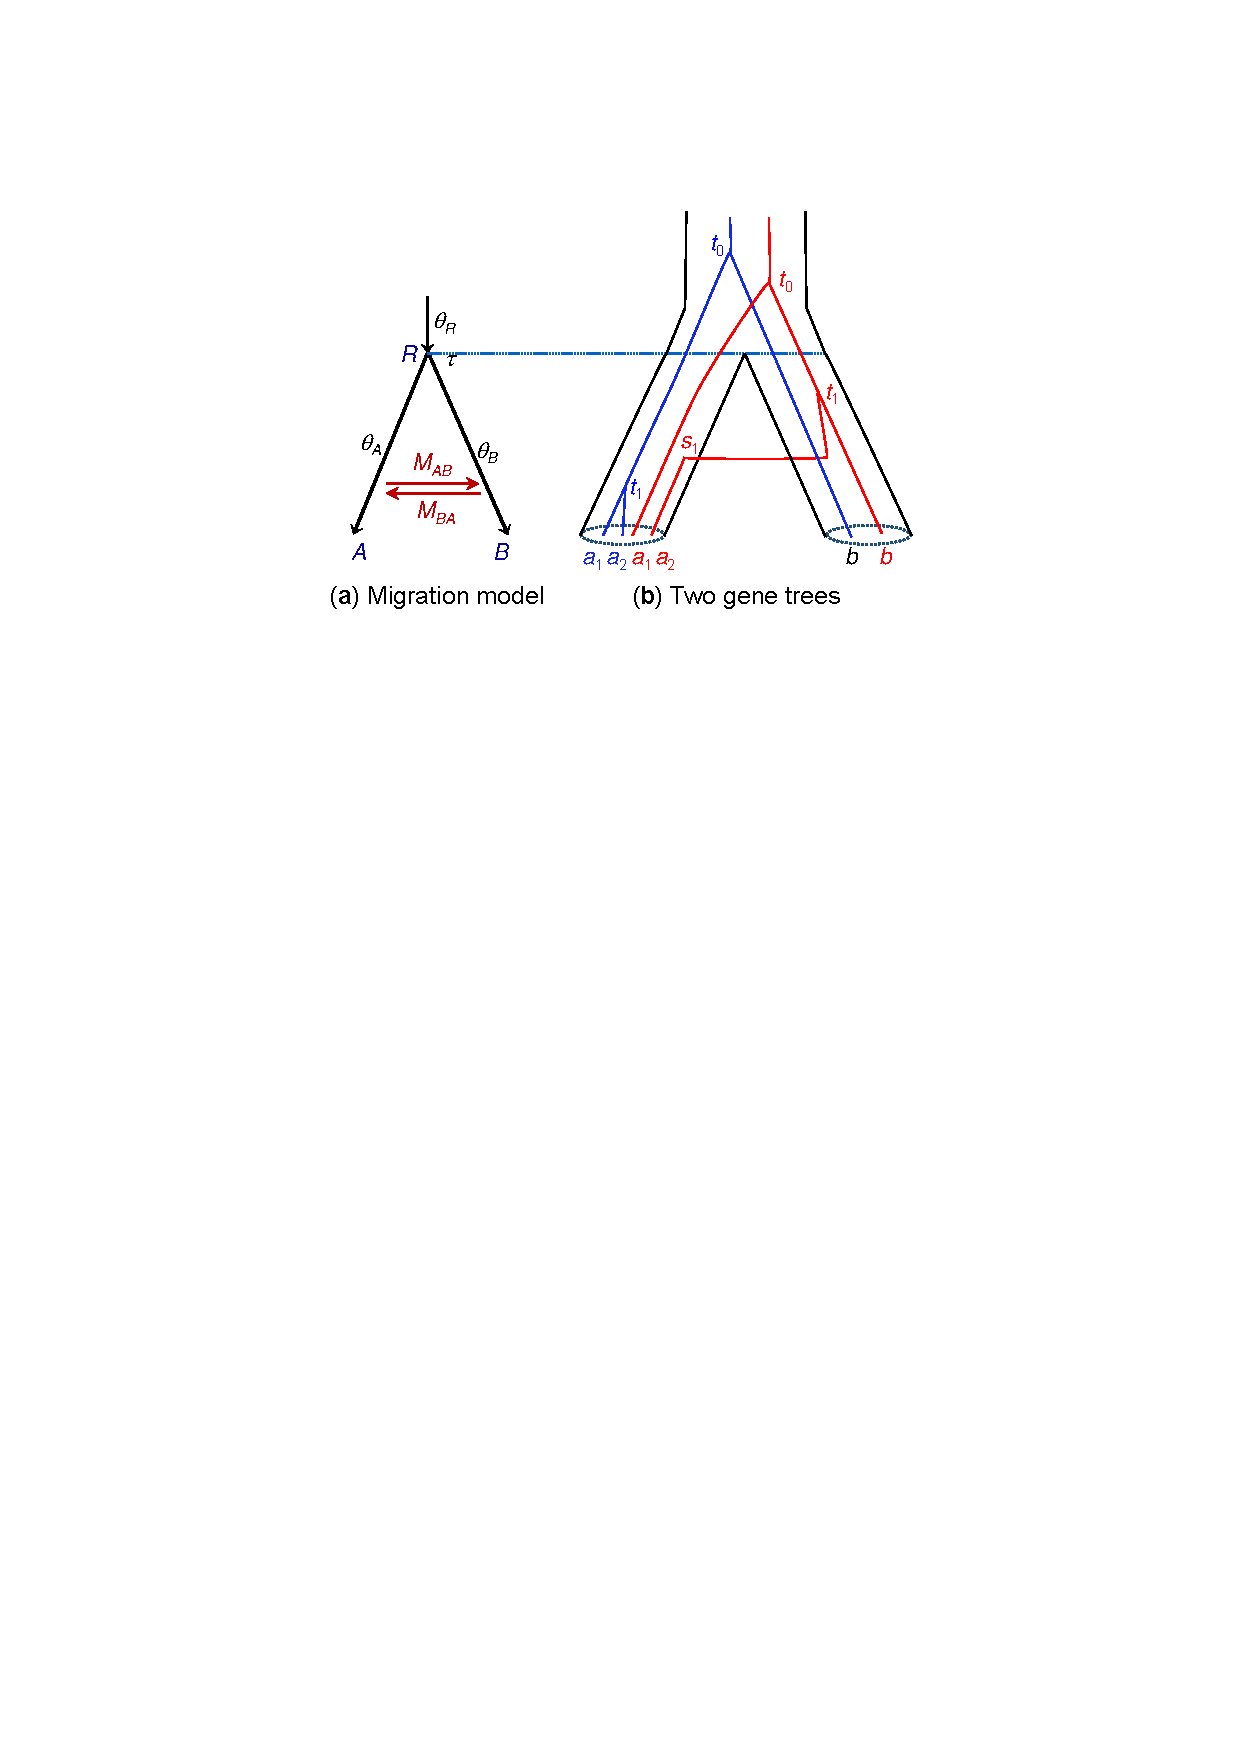
\includegraphics[scale=0.6]{figs/fig-tree-mscm} %
   
   \caption{(\textbf{a}) An MSC-with-migration (MSC-M) model for two species or
      populations ($A,B$) showing the parameters.  The two species diverged time $\tau
      \equiv \tau_{AB}$ ago and have since been exchanging migrants at the rate of $M_{AB}
      = m_{AB}N_B$ migrants per generation from $A$ to $B$ and at the rate $M_{BA}$ from
      $B$ to $A$.  (\textbf{b}) Two gene trees at two loci, each with two sequences ($a_1,
      a_2$) from population $A$ and one sequence ($b$) from $B$.  In the blue tree,
      sequences $a_1$ and $a_2$ coalesce first, in population $A$, resulting in the gene
      tree $G_1 = ((a_1,a_2),b)$.  In the red tree, sequence $a_2$ migrates into
      population $B$ and coalesce with sequence $b$ in population $B$, resulting in the
      gene tree $G_2 = ((a_2,b),a_1)$.  The \textit{gdi} index is defined as the
      probability that the first coalescence occurs between the two $A$ sequences and
      before reaching species divergence when we trace the genealogy backwards in time. %
   } \label{fig:tree-mscm}
\end{figure}

Under the MSC-M model, the \textit{gdi} can be computed analytically, using the Markov
chain characterization of the backward-in-time process of coalescent and migration
\citep{Leache2019}.  For two populations ($A$ and $B$) with gene flow and three
sequences ($a_1$, $a_2$, and $b$), the genealogical process of coalescent and migration
when one traces the history of the sample backwards in time can be described by a Markov
chain.  The state of the chain is specified by the number of sequences remaining in the
sample and the population IDs ($A$ and $B$) and the sequence IDs ($a_1, a_2, b$, etc.). 
For example, The initial state is $A_{a_1}A_{a_2}B_b$, in which three sequences $a_1,
a_2, b$ are in populations $A$, $A$, and $B$, respectively.  This is also written as
`$AAB$'.  State $A_{a_1a_2}B_b$, abbreviated `$AB_b$', means that two sequences remain
in the sample, with the ancestor of sequences $a_1$ and $a_2$ in population $A$ and
sequence $b$ in population $B$.  There are 21 states in the Markov chain.

The transition rate matrix of the Markov chain $Q = \{q_{ij}\}$ is given in
table~\ref{table:Q}. The transition probability matrix over time $t$ is then $P(t) =
\{p_{ij}(t)\} = \e^{Qt}$, where $p_{ij}(t)$ is the probability that the Markov
chain is in state $j$ at time $t$ in the past given that it is in state $i$ at time 0 (the
present time).  Suppose $Q$ has the spectral decomposition
\begin{equation} 
    q_{ij} = \sum_{k=1}^{21} u_{ik} v_{kj} \lambda_k ,
\end{equation} 
where $0 = \lambda_1 > \lambda_2 \ge \cdots \ge \lambda_{21}$ are the eigenvalues of
$Q$, and columns in $U = \{u_{ij}\}$ are the corresponding right eigenvectors, with $V =
\{v_{ij}\} = U^{-1}$.  Then
\begin{equation} \label{eq:pij}
    p_{ij}(t) = \sum_{k=1}^{21}  u_{ik} v_{kj} \e^{\lambda_k t}.
\end{equation}

Consider the coalescent time $t$ between sequences $a_1$ and $a_2$ given that they are to
coalesce first and before $\tau$ (as in the blue gene tree of fig.~\ref{fig:tree-mscm}b).
This has density
\begin{equation} \label{eq:ft} 
\begin{aligned}
  f(t) &= \bigl[ p_{AAB, AAA}(t) + p_{AAB, AAB}(t) \bigr] \tfrac{2}{\theta_A} \\
       &+ \bigl[ p_{AAB, BBA}(t) + p_{AAB, BBB}(t) \bigr] \tfrac{2}{\theta_B}, \ \ t < \tau.
\end{aligned}
\end{equation} 
The two terms in the sum correspond to coalescence between $a_1$ and $a_2$ occurring in
populations $A$ and $B$, respectively.  The first term is the probability, $p_{AAB,
   AAA}(t) + p_{AAB, AAB}(t)$, that sequences $a_1$ and $a_2$ are in $A$ right before time
$t$, times the rate for them to coalesce $\bigl( \frac{2}{\theta_A} \bigr)$. Similarly
the second term is the probability density that $a_1$ and $a_2$ coalesce at time $t$ in
$B$.

By averaging over the distribution of $t$, we have 
\begin{equation} \label{eq:gdi} 
    gdi = \int_0^\tau f(t) \; \d t ,
\end{equation}
where $f(t)$ is given in eq.~\ref{eq:ft}. To calculate the integral in eq.~\ref{eq:gdi},
note that from eq.~\ref{eq:pij},
\begin{equation} 
   \begin{aligned}
      \int_0^\tau p_{ij}(t) \,\d t = 
       u_{i1} v_{1j}\tau %
       + \sum_{k=2}^{21} u_{ik} v_{kj} \frac{\e^{\lambda_k \tau} - 1}{\lambda_k} .
   \end{aligned}
\end{equation}

We have implemented this calculation of the \textit{gdi} in the python pipeline for the
case where the two populations are sister lineages exchanging migrants between
themselves but not with other populations.

When populations $A$ and $B$ are involved in gene flow with other populations,
analytical calculation of the $gdi$ becomes complicated.  It is simpler to simulate gene
trees for sequences $a_1, a_2, b$ under the extended migration model involving more than
two populations to calculate the \textit{gdi}.  Specifically, given the fully specified
MSC-M model for all species/populations (including the species tree topology and
parameters such as $\tau$, $\theta$, $M$), simulate the gene trees with branch lengths
(coalescent times) for a large number of loci ($R = 10^6$, say) , at which three
sequences ($a_1, a_2, b$ ) are sampled.  The $gdi$ is simply the proportion of loci at
which the gene tree is $G_{1a}$, that is, $G_1$ with $t_1 < \tau_{AB}$
(fig.~\ref{fig:gdi-trees}).



\section{The hierarchical merge and split algorithms}

\begin{figure}
   \centering %
   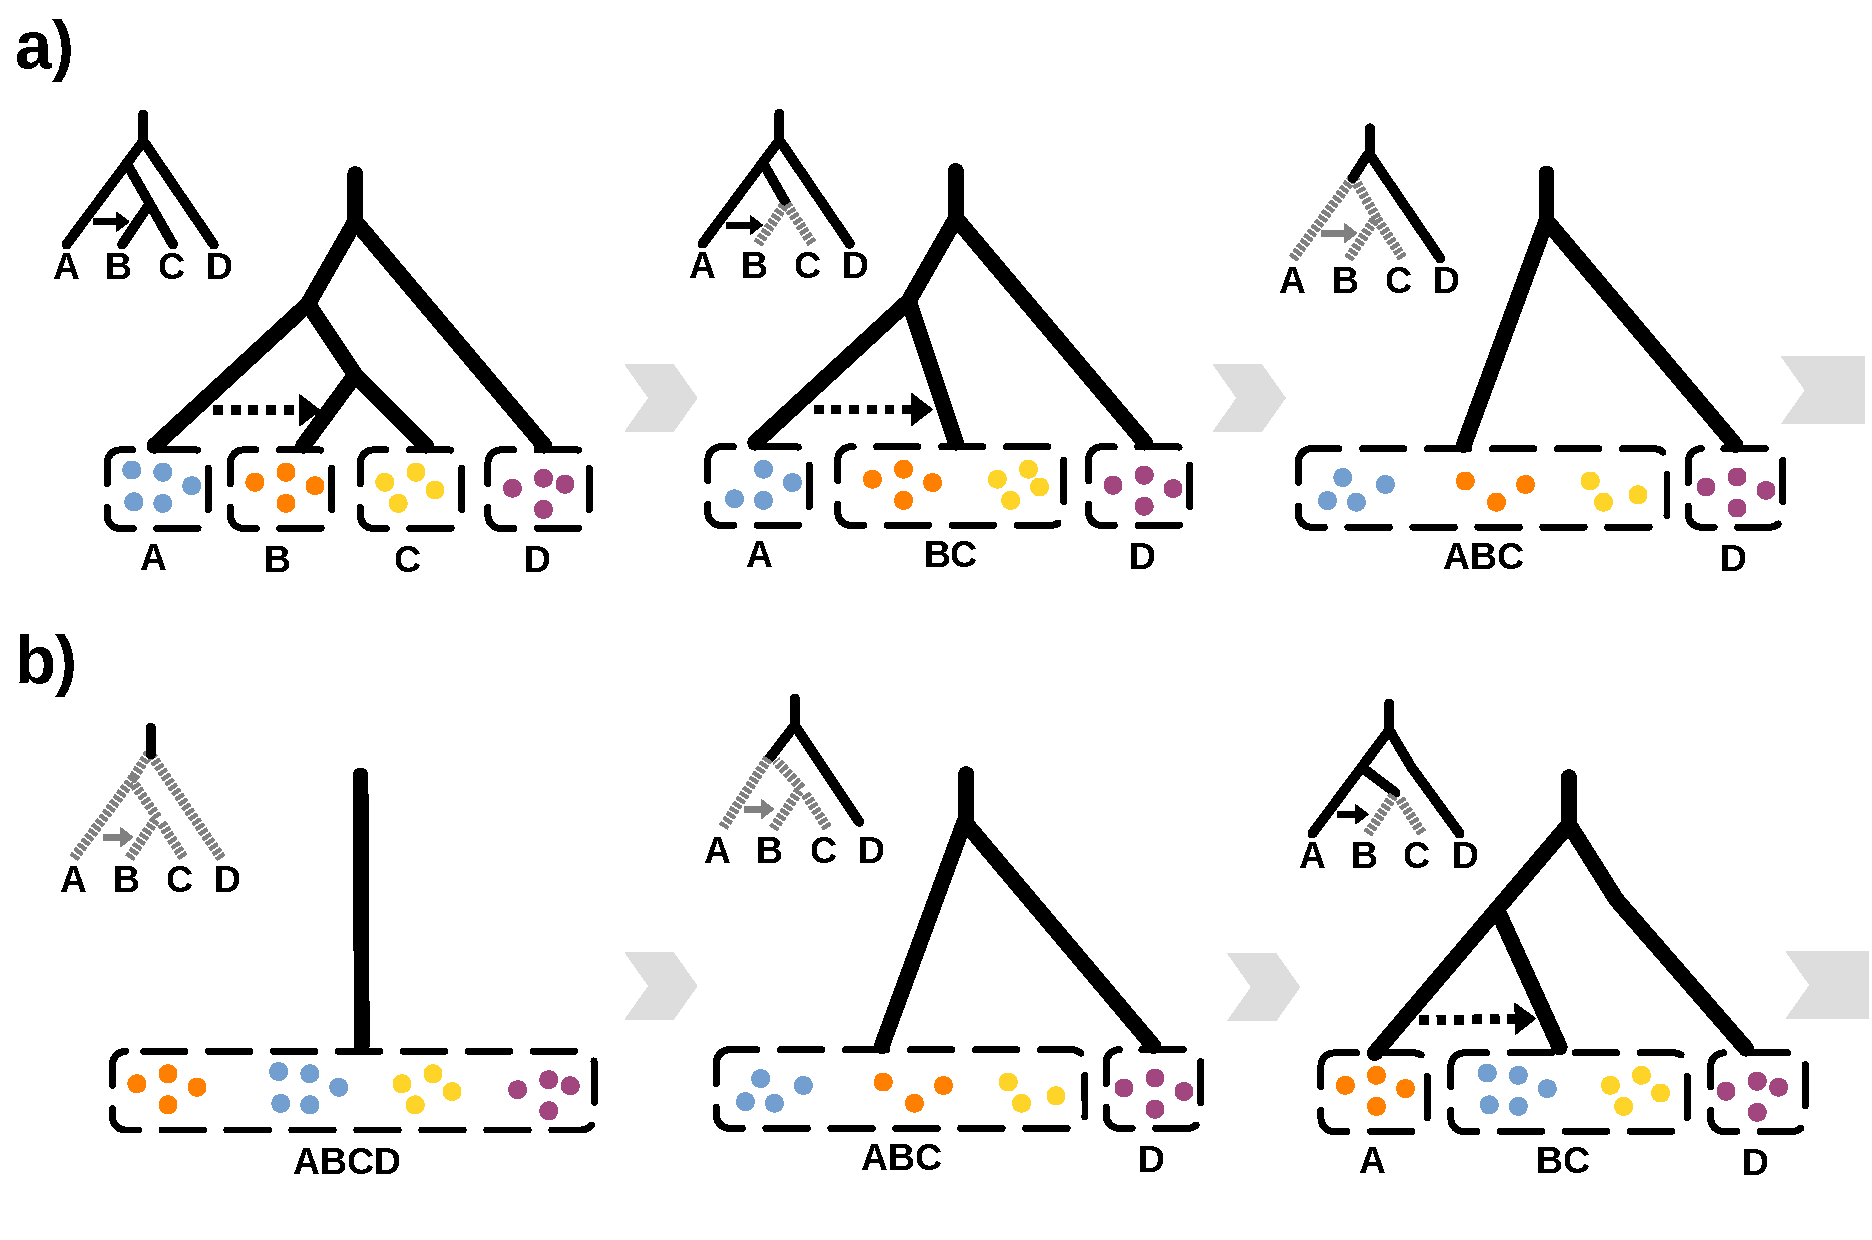
\includegraphics[scale=0.25]{figs/Methods/HM_algo} %
   
   \caption{(\textbf{a}) Hierarchical merge and (\textbf{b}) hierarchical split
   algorithms applied to the same guide tree for four populations. \\%
	} 
	\label{fig:gdi-algorithms}
\end{figure}

We implement both the hierarchical merge and hierarchical split algorithms in a python
pipeline (fig.~\ref{fig:gdi-algorithms}).  Both algorithms require a guide tree for
populations, possibly with migration events.  In the merge algorithm, we progressively
merge the populations into the same species, starting from the tips of the tree and moving
towards the root.  The merge is accepted if and only if the \textit{gdi} $< 0.2$ for the
population pair.  The algorithm stops when no population/species pair can be merged
(fig.~\ref{fig:gdi-algorithms}a).

In the hierarchical split algorithm, we start from the MSC model of one species and
progressively split each species into distinct species, starting from the root and moving
towards the tips of the tree (fig.~\ref{fig:gdi-algorithms}b).  The split is accepted if and
only if the \textit{gdi} $> 0.7$ for the species pair.  The algorithm stops when no
species can be split (fig.~\ref{fig:gdi-algorithms}b).

If there are $K$ populations on the guide tree, the merge algorithm arrives at a high
number of species while the split algorithm arrives at a low number, with $1 \le K_l \le
K_u \le K $.

\clearpage
\newpage

\section{Example with simulated data ($ABCDX$)}

\begin{figure}[h]
   \centering
   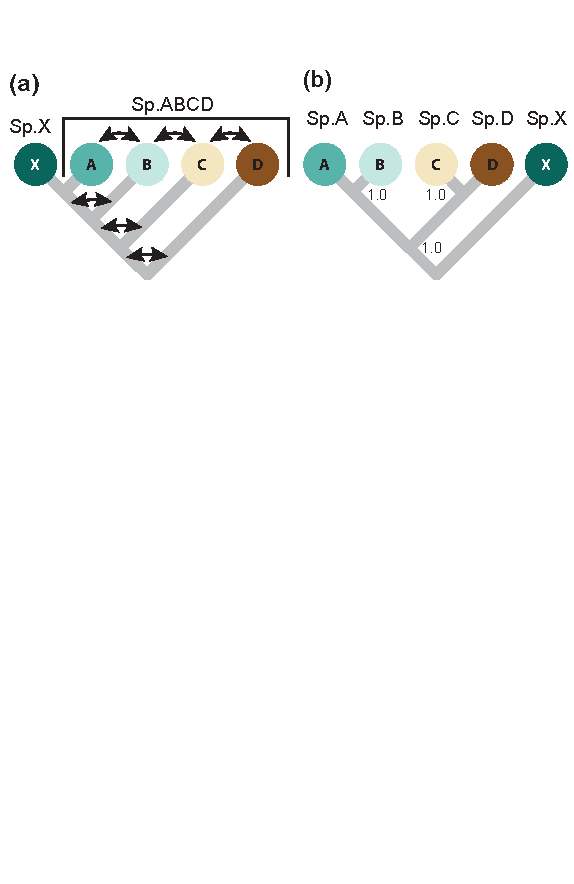
\includegraphics[scale=0.7]{figs/fig-ABCDX}
   
   \caption{(\textbf{a}) An isolation-by-distance model used to simulate multilocus
    sequence data.  $A, B, C, D$ represent populations of a widely distributed species
    while $X$ is a new species that split off from population $A$.  (\textbf{b}) Incorrect
    species delimitation and phylogeny in Bayesian model selection using \textsc{bpp} under
    the MSC model assuming no gene flow.  Use of the guide tree and the \textit{gdi}
    criterion leads to delimitation of two species.  Redrawn after
    \citet[][fig.~5]{Leache2019}. %
} \label{fig:ABCDX}
\end{figure}

\citet{Leache2019} simulated sequence data under the MSC-with-migration model for five
populations (fig.~\ref{fig:ABCDX}).  Populations $A, B, C, D$ represent a single
large paraphyletic species distributed across a wide geographic range.  Migration
between any two neighbouring populations occurs at the rate of $M = Nm = 2$ migrants per
generation. $X$ represents a new species that split off from population $A$, and there
is no gene flow to or from $X$.  The data consisted of $L=100$
simulated loci, with two sequences sampled per species per locus, and 500 sites in the
sequence.  We use the dataset to illustrate our pipeline. 

The complete master control file for the program can be found in \ref{fig:ABCDX_mcf}. 
During the analysis, the pipeline provides written feedback to the user about the current state of the
delimitation and the decisions made during each iteration (\ref{fig:ABCDX_text_out}).
This is accompanied by visualisations of the species delimitation and the decision process (Fig. \ref{fig:ABCDX_out}).

During the first iteration of the iterative refinement, the pipeline proposes to merge the
two current leaf node pairs (A-B, C-D).As the gdi values for the population pairs were below the 0.2 threshold, the A-B and C-D population pairs are
merged. During the second iteration, the pipeline proposes to merge the AB-CD population pair. 
During the third iteration, the pipeline proposes that the ABCD-X population pair could be
merged. However, after calculating the gdi values, the proposal is rejected and the final delimitation is reached. 
The final species delimitation (ABCD, X), is the known correct solution.

\begin{figure}[h]
	\begin{center}
		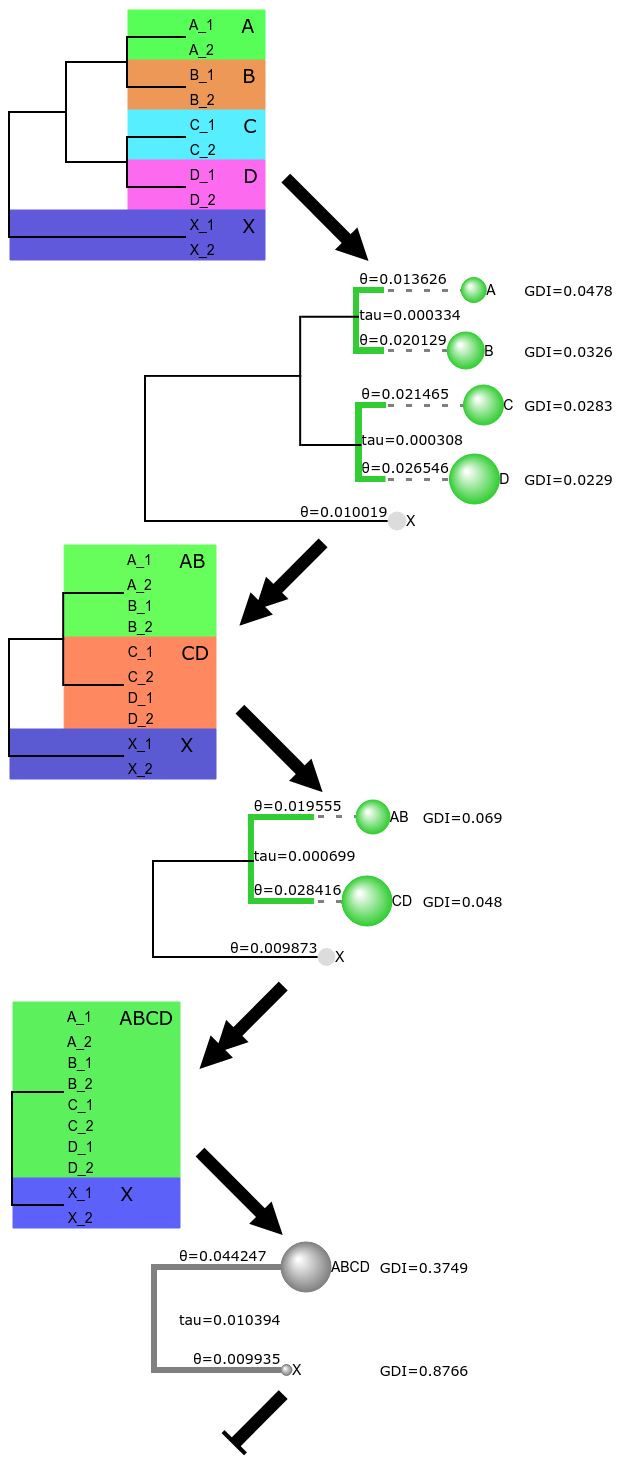
\includegraphics[scale=0.35]{figs/Pipedemo/sim_fig_v1}
	\end{center}
	\caption{Visual feedback produced by the pipeline during the three iterations. Visualisations of the currently accepted species delimitation are in the left column. Visualisation of the changes to the phylogenetic tree are in the left column}
	\label{fig:ABCDX_out}
\end{figure}

\clearpage
\newpage
\section{Empirical examples}

\subsection{Species delimitation in the genus Giraffa}

\begin{figure}[t]
    \centering %
    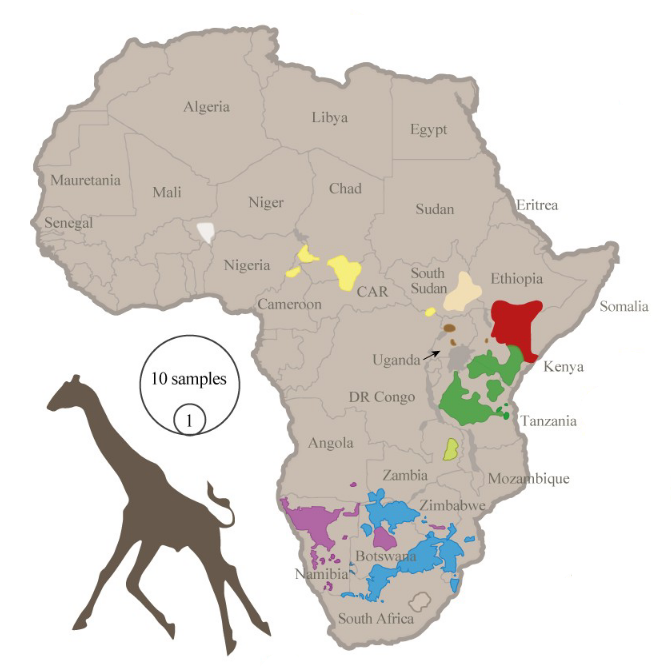
\includegraphics[scale=0.25]{figs/fig-giraffe} %
    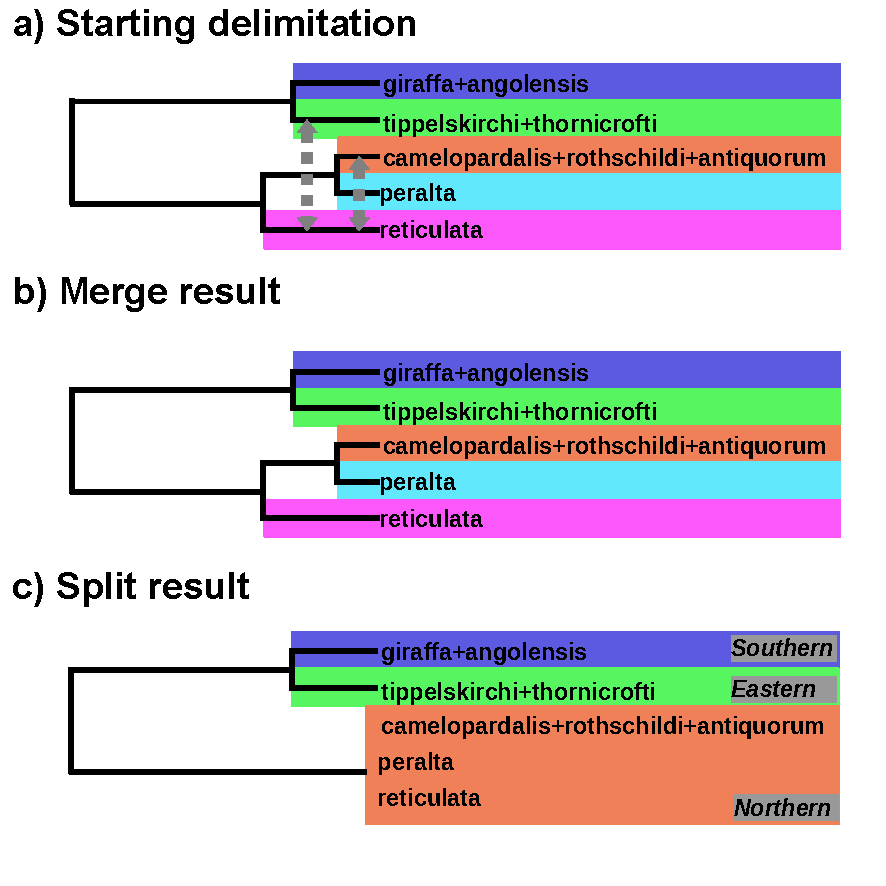
\includegraphics[width=\linewidth]{figs/Giraffe/giraffe_progress_vector}  %
    
    \caption{(\textbf{a}) The geographical distributions of nine subspecies of
   giraffa, modified from \citet{Petzold2020}, figure.  (\textbf{b}) The hierarchical
   split algorithm supports 3 species, while (\textbf{c}) The hierarchical merge
   algorithm supports 5 species.
} \label{fig:giraffe}
\end{figure}

Species delimitation in the genetically isolated, but
phenotypically convergent Giraffes has generated
sizeable controversy (Fišer et al., 2018). Based
on morphological characters and molecular data,
various hypotheses have classified the nine giraffe
subspecies ( \textit{camelopardalis},
\textit{angolensis}, \textit{antiquorum}, \textit{giraffa}, \textit{peralta},
\textit{reticulata}, \textit{rothschildi}, \textit{thornicrofti} and
\textit{tippelskirchi}. ) into anywhere from one to six species.

\citet{Petzold2020} compiled a multilocus dataset of 21 introns (average sequence length
808 bp), sampled from 66 individuals from the nine subspecies.  They found that
population genetic approaches, such as the program \textsc{structure} and the
phylogenetic approaches implemented in MrBayes, PhyML, and SuperTRI all supported three
species. However, the MSC based methods in *BEAST, STACEY, and \textsc{bpp} strongly
supported five species. 


Based on the observations of mitochondrial haplotypes and
hybridized individuals \citep{Fennessy2016, Petzold2020}, bidirectional migration was
specified between the \textit{tippelskirchi} and \textit{reticulata}, as well as the
\textit{reticulata} and \textit{rothschildi} subspecies.  The migration rate was assigned
the prior ($\Gamma (1,100)$) with mean 0.01 migrant individuals per generation.  Merge and
split analyses were conducted with the animal specific $gdi$ thresholds of 0.3 and 0.7, as
recommended by \citet{Jackson2017} (master control files available in \ref{fig:giraffe_mcf_merge} and \ref{fig:giraffe_mcf_split})..

The split algorithm suggested three species while the merge
algorithm suggested five (fig.~\ref{fig:giraffe}).  Both grouped the Eastern populations
\textit{thornicrofti} and \textit{tippelskirchi} into one species, and the Southern
populations \textit{angolensis} and \textit{giraffa} into another species. The split
algorithm lumped the remaining five subspecies into a single Northern species, while the
merge algorithm recognized four species. 



\newpage
\subsection{Species delimitation in milksnakes (\textit{Lampropeltis triangulum})}

\begin{figure}
    \centering %
    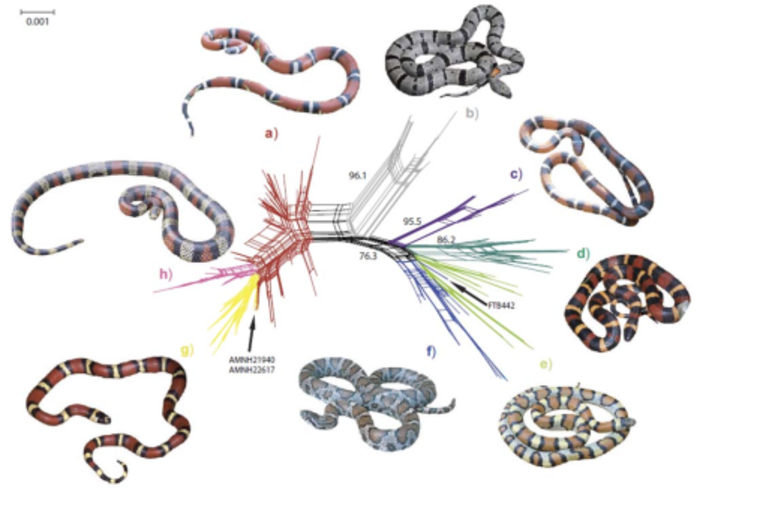
\includegraphics[scale=0.5]{figs/miksnakes} %
    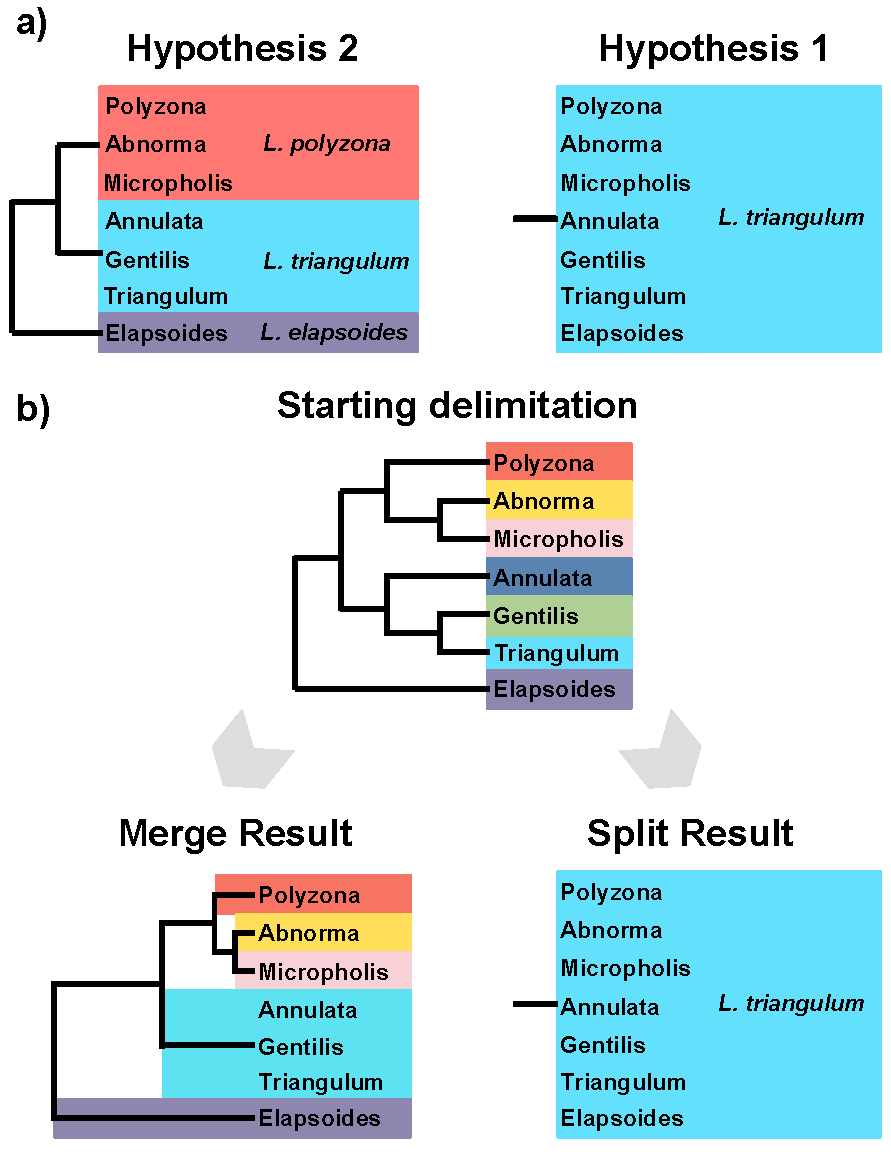
\includegraphics[scale=0.5]{figs/fig-miksnakes-results} %
    
    \caption{\textbf{Top:} Species delimitation hypotheses in \textit{Lampropeltis triangulum}.
    \textbf{a)} Three-species, and one-species delimitation hypotheses suggested by
    \citet{Chambers2020}.  \textbf{b)} Starting delimitation, and results from merge and
    split analysis. \\ %
} \label{fig:milksnake}
\end{figure} 

The  American milksnake \textit{Lampropeltis triangulum} is a New World snake with one of
the widest known geographic distributions within the squamates, with seven subspecies
known: \textit{abnorma}, \textit{polyzona}, \textit{micropholis}, \textit{triangulum},
\textit{gentilis}, \textit{annulata}, \textit{elapsoides} (fig.~\ref{fig:milksnake}a).  
\citet{Ruane2014} analyzed 11 nuclear loci (average length 537 bp) for 164 individuals
from the seven subspecies using \textsc{bpp} and found evidence for seven independent
species. 

\citet{Chambers2020} criticised these results, suggesting that several of the
hypothesized species of milksnakes appear to represent arbitrary slices of continuous
geographic clines.  Based on a combination of phylogeographic and genetic evidence, they
suggested two alternative hypotheses: a one-species hypothesis merging all subspecies into
a single species, or a three-species hypothesis separating the \textit{polyzona},
\textit{triangulum}, and \textit{elapsoides} lineages as species. 

Chambers and Hillis (2020) also demonstrated that
five different arbitrary east-west splits of the the
\textit{gentilis} and \textit{ triangulum} populations are all supported
by BPP as being two separate species (Fig. 7). This
result is highly concerning, as these five alternative
species delimitations are not mutually compatible.
These results also echo the simulations of \cite{Barley2018}, who demonstrated that BPP will delimit
geographically separated clusters of individuals from
a single species as distinct species entities.

We analyzed the data using our pipeline, using the guide tree of \citet{Chambers2020}, with no migration
rates assumed (fig.~\ref{fig:milksnake}).  Merge and split algorithms were run using $gdi$
thresholds of 0.3 and 0.7 (master control files available in \ref{fig:milksnake_mcf_merge} and \ref{fig:milksnake_mcf_split}).

The merge algorithm established an upper bound of five species.  When compared with the
three-species hypothesis that was the suggested upper bound by \citet{Chambers2020}, two
of the species (\textit{elapsoides} and \textit{triangulum}) were identical, but
HMDelimit identified additional diversity in the \textit{polyzona} branch, marking each
population as a distinct species.  The split analysis only supported a single species.

\begin{figure}
	\centering %
	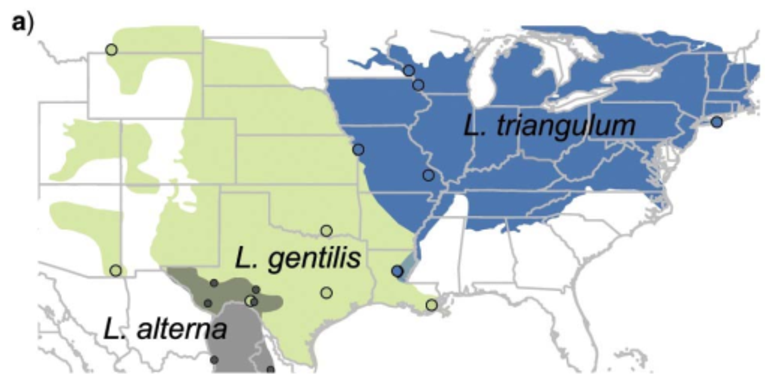
\includegraphics[scale=0.5]{figs/miksnakes_EW} %
	
	\caption{East-West splits. Coloured dots represent the sampling location and original classification of
		individuals (blue: \textit{triangulum}, green: \textit{gentilis}). %
	} \label{fig:milksnake_EW}
\end{figure} 

We conducted a second analysis using only the 38 individuals from the \textit{gentilis},
\textit{triangulum}, and \textit{alterna} populations (which acted as an outgroup in all
analyses).  The assignment of individuals to the \textit{gentilis} and \textit{triangulum}
populations was varied in each analysis, according to the five arbitrary East-West splits of \cite{Chambers2020} (fig.~\ref{fig:milksnake}). 
Merge and split analyses were ran using the settings as above (master control files available in \ref{fig:milksnake_EW_mcf} and \ref{fig:milksnake_EW_shell}). 

For all five of the East-West geographic splits tested, our merge and split analyses converged on an identical result,
merging the \textit{gentilis} and \textit{triangulum} populations into a single species, congruent with the suggestions of \cite{Chambers2020}.



\subsection{Introgression and species delimitation in the longear sunfish (\textit{Lepomis megalotis}).}

\begin{figure}[t]
    \centering %
    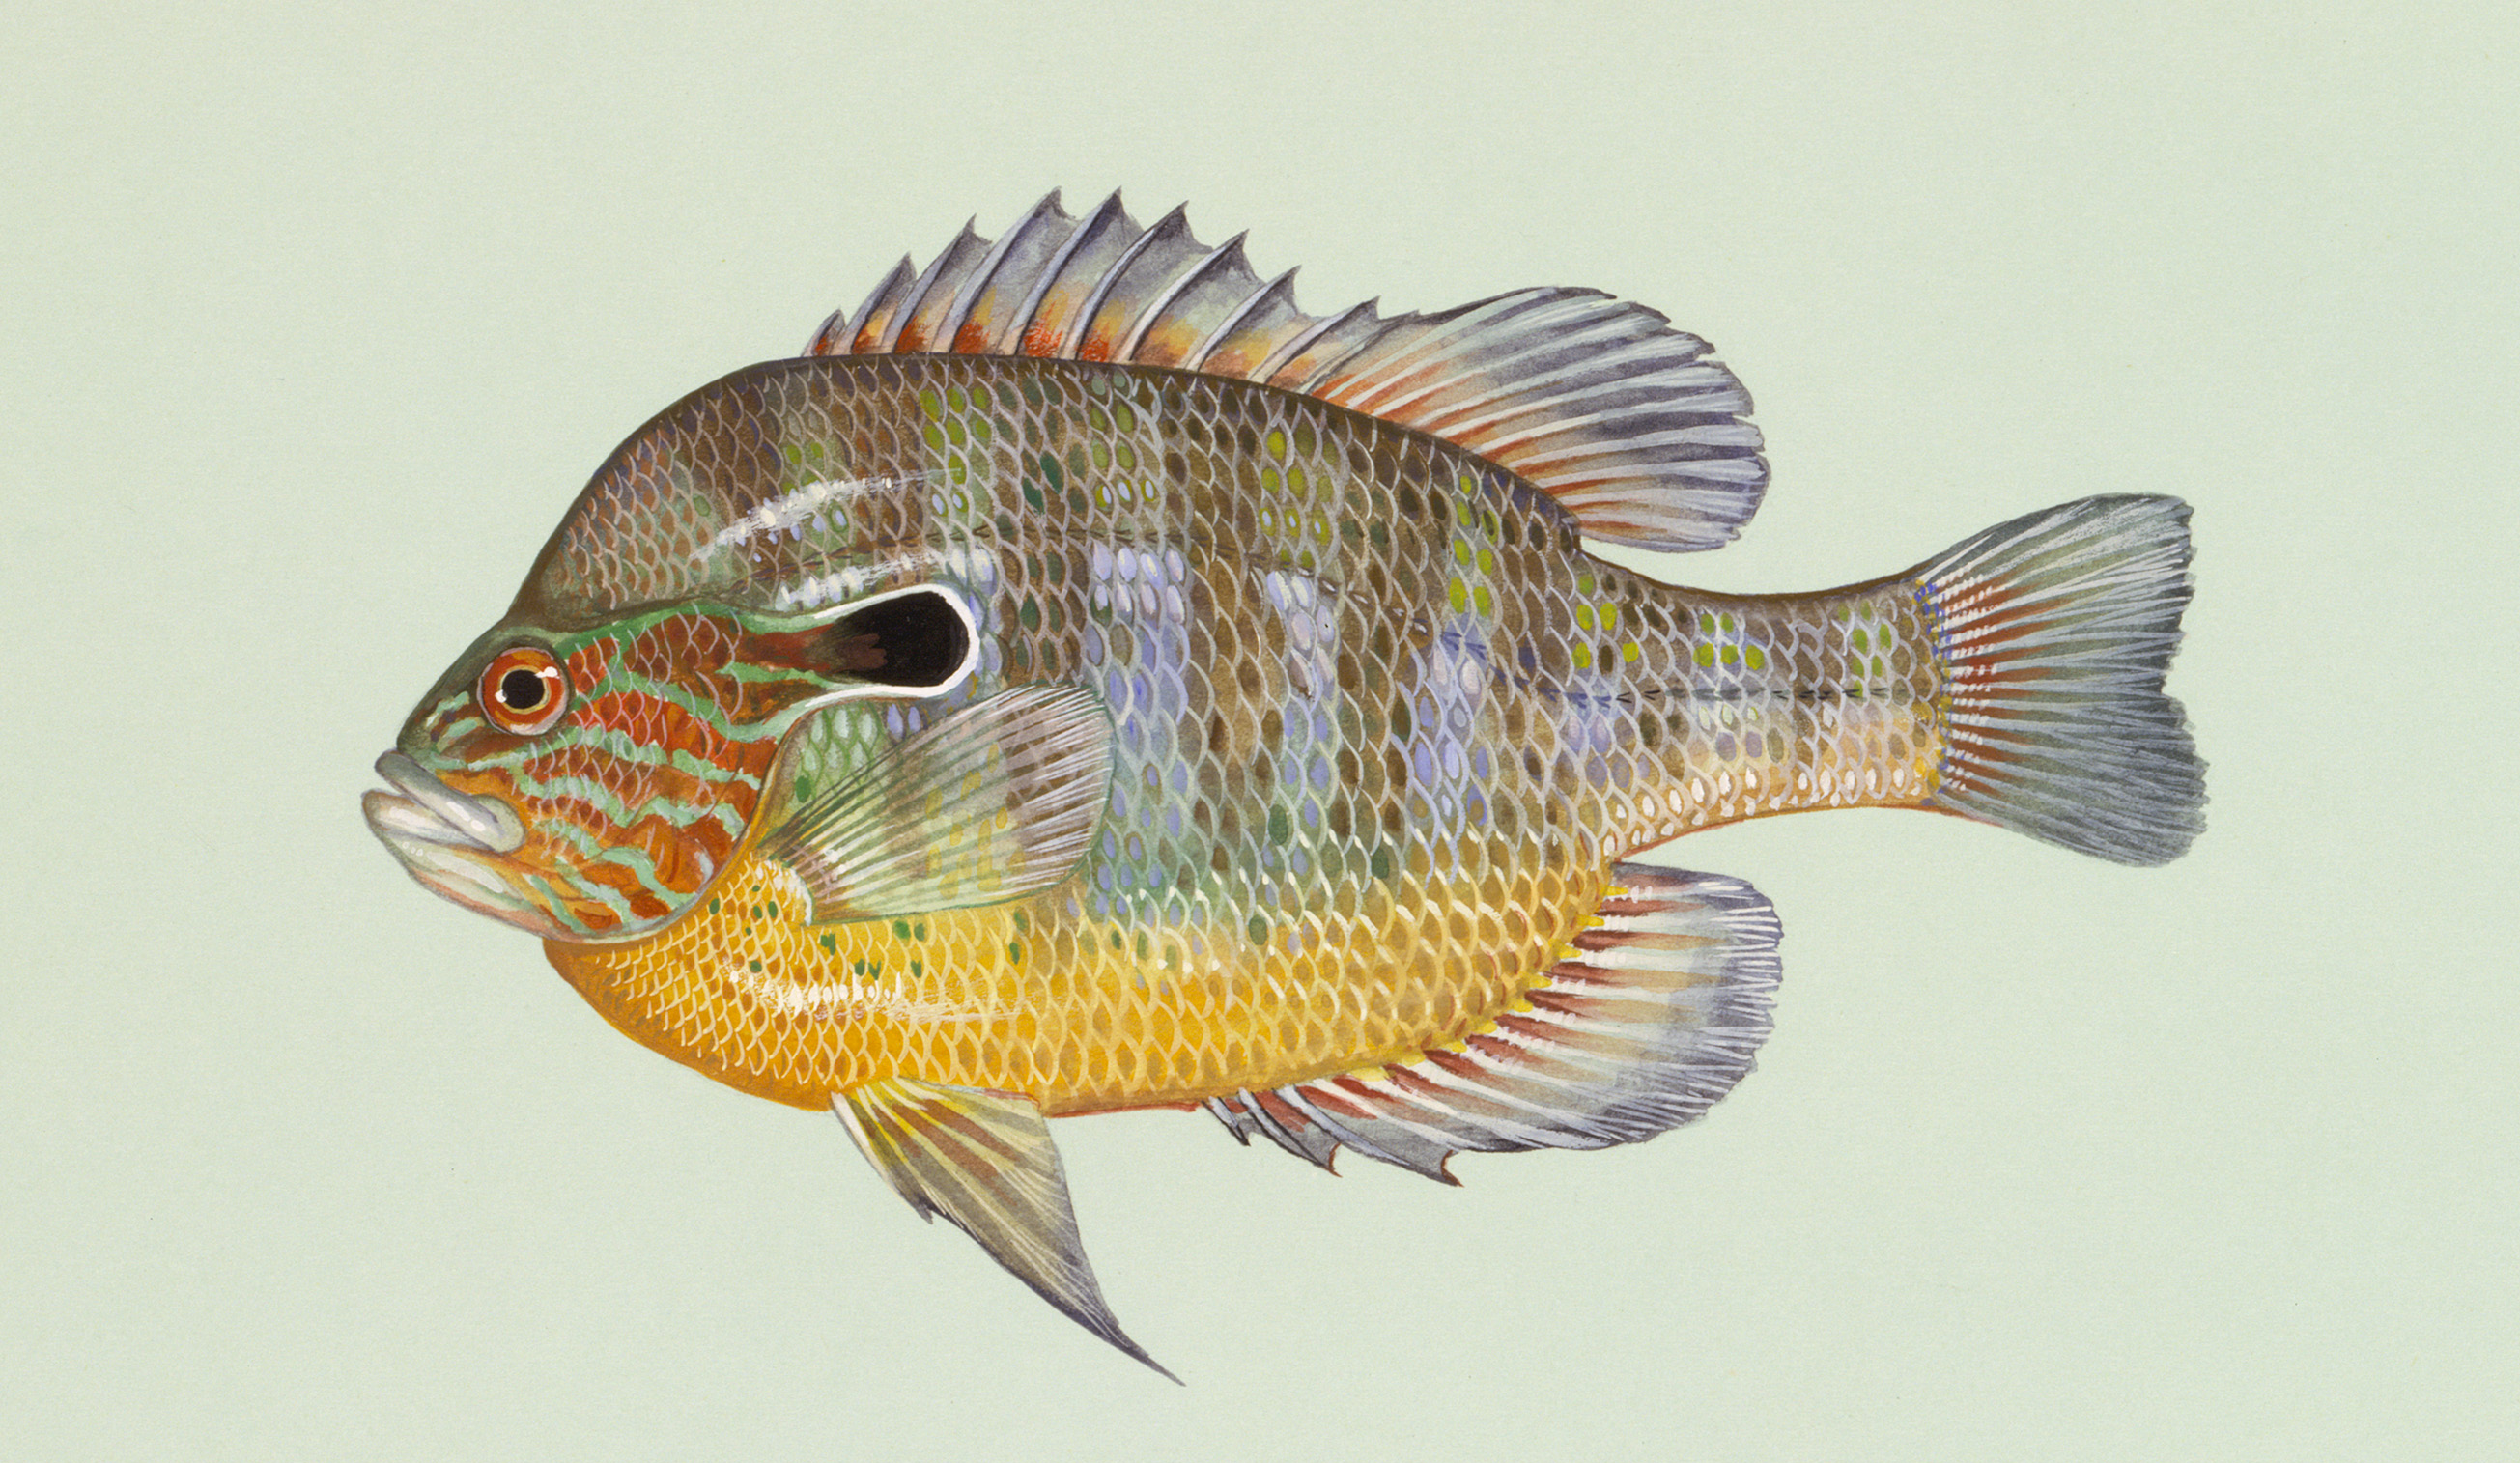
\includegraphics[scale=0.3]{figs/Sunfish/Lepomis_megalotis}
    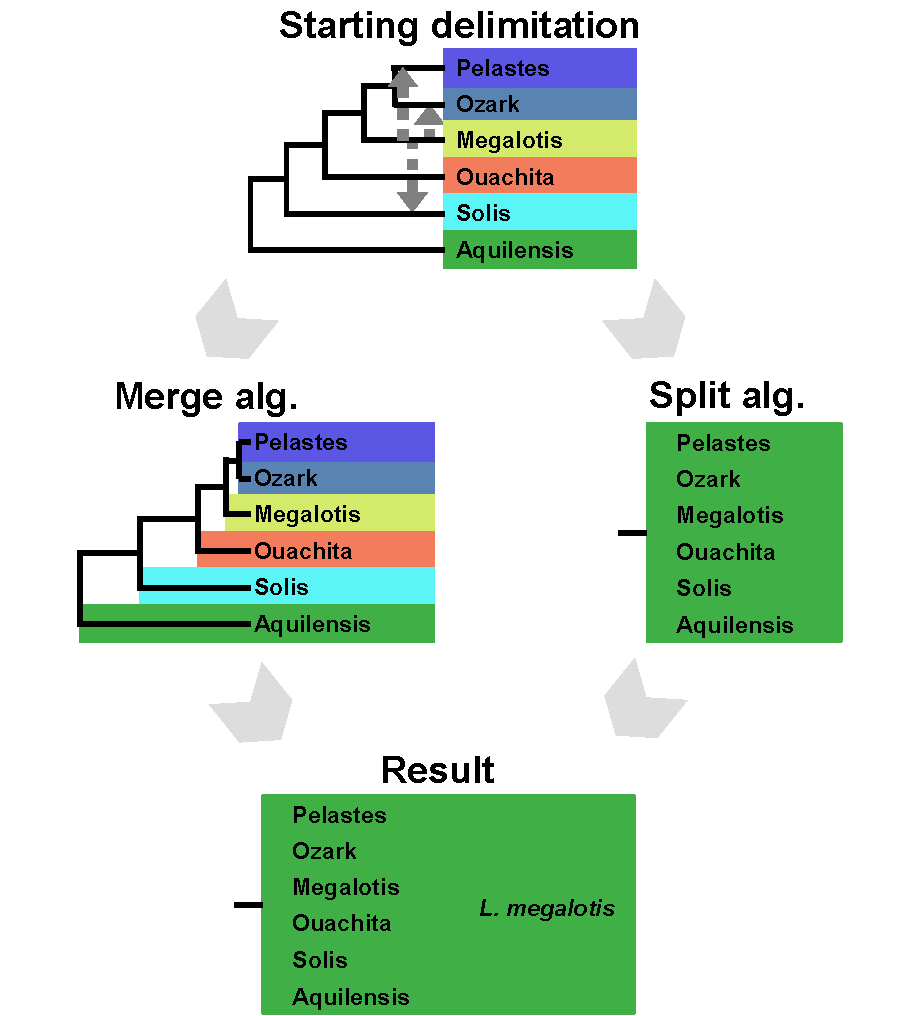
\includegraphics[scale=0.5]{figs/fig-longear-fish-results}
    
    \caption{Species delimitation in the Longear Sunfish \textit{Lepomis megalotis}.
        Both the merge and split algorithms support a single species. %
    } \label{fig:sunfish}
\end{figure}

The longear sunfish (\textit{Lepomis megalotis}) is a freshwater fish in the sunfish
family, Centrarchidae, of order Perciformes.  It is native to eastern North America from
the Great Lakes down to northeastern Mexico.  Due to widespread geographic distributions
and frequent hybridizations, species delimitation in the longear sunfish poses
considerable challenges. 

\citet{Kim2022} analyzed a dataset of 163 ddRAD loci (average
sequence length 89 bp) sampled from 50 individuals from the six subspecies:
\textit{aquilensis}, \textit{solis}, \textit{ouachita}, \textit{megalotis},
\textit{ozark}, \textit{pelastes}.  After determining a species tree using
\textsc{IQ-tree}, they used \textsc{bpp} A00 without migration to calculate $\tau$ and
$\theta$ parameters for each of the subspecies, and used these values to calculate
\textit{gdi} scores, and delimit species in the group. They found that none of the populations have \textit{gdi} values supporting distinct species status. \citet{Kim2022} also utilized \textsc{Fastsimcoal2} to identify patterns
of gene flow, and find evidence for multiple instances of significant historical or
ongoing genetic exchange.  This may be problematic, as their genetic delimitation procedure
did not account for the patterns of gene flow observed.

We reanalyzed the data, taking into account migration between the subspecies.  Based on the hybridization patterns observed by \cite{Kim2022}, migration from the \textit{megalotis} population to
the \textit{pelastes}, \textit{solis}, and \textit{ozark} populations was specified. The migration rate was assigned
the prior ($\Gamma (1,100)$) with mean 0.01 migrant individuals per generation. Merge and split algorithms were run using $gdi$
thresholds of 0.3 and 0.7 (master control files available in \ref{fig:sunfish_mcf_merge} and \ref{fig:sunfish_mcf_split}).

Both merge and split analyses supported a single species.  This is congruent with the $gdi$
based delimitation of \citet{Kim2022}, who found that all populations have $gdi$ values
below the threshold for distinct species status.


\newpage
\section{Discussion}

\subsection{Challenges of heuristic species delimitation}

Several issues with the \textit{gdi} criterion have been noted before \citep{Leache2019}.  
First, given populations $A$ and $B$, two \textit{gdi} values may be calculated:
\begin{equation}
   \begin{aligned}
      gdi_A = 1 - \e^{-2\tau _{AB}/\theta_A} \\
      gdi_B = 1 - \e^{-2\tau _{AB}/\theta_B}
   \end{aligned}
\end{equation}
These may not be consistent concerning the species status of populations $A$ and $B$
\citep{Leache2019}.

Second, the \textit{gdi} may be large because the population is very small.
\citet{Rannala2020} recommended the use of absolute divergence time, such that two
populations are considered distinct species only if their \textit{gdi} $> 0.7$.

\textbf{Assignment of individuals to populations and construction of the guide tree.}
Our pipeline requires the user to supply a guide tree.  This may be inferred using a
species tree estimation method under the MSC model with no gene flow \citep{Yang2014,
   Rannala2017}.  Alternatives include maximum likelihood tree inference using concatenated
data, or use of the mitochondrial genes.

The arbitrariness of the criterion.  However, for mammals, a 10\% CO1 (or cytb)
divergence is a sure thing for distinct species.

Any empirical thresholds for particular criteria or properties will be imprecise, as it
is recognized by multiple authors that such an attempt is futile \cite{Wells2022}. While
there can be no set of universal criteria or properties applicable to species
delimitation, a heuristic approach does provide useful guide.

Molecular phylogenetic or population genetic analysis should always be integrated with
an assessment of congruence with morphological and ecological data.  Using genetic data,
one should not exclude species generated by processes that do not automatically or
immediately result in monophyly, such as hybrid speciation, polyploidy, or paraphyly in
the case of recent ancestor-descendant speciation.  Where molecular phylogenetic
analysis is impractical due to inadequate samples or easily sequenced material, or where
it fails to resolve well-supported relationships, species delimitation remains possible,
but should be based on a strong hypothesis of phylogenetic relatedness resulting from
multiple and unambiguous phenotypic and ecological traits.

The effects of sampling.  Many empirical biologists emphasized the importance of
sampling: \citet{Chambers2020, Wells2022}.  \cite{Yang2017} has pointed out that rarity
and singletons should not be a major problem. Migration rates can also be estimated when
some species are missing or unsampled. \citet{Zhang2011} through simulation illustrated
that failure to sample the intermediate populations in a stepping-stones design does not
cause false positives for species delimitation by \textsc{bpp}.


\subsection{Gene flow and non-monophyletic species}

Analyses of genomic data in the past two decades have demonstrated the prevalence of
interspecific gene flow.  Several studies suggested evidence for speciation despite
ongoing gene flow, as in \textit{Heliconius} butterflies \citep{Martin2013}, Mangrove
trees \citep{He2019}, and Western Pacific abalones \citep{Hirase2021}.  Issues arise
when we want to delimit species when there is gene flow between the species or
populations.

\textit{Bayesian model selection.}  First consider Bayesian model selection. There are
three models for two populations ($A,B$): M1: one species, M2-0 two species with no
migration, and M2-m two species with migration.  \citet{Leache2019} compare M1 and M2-0 to
decide whether there are one or two species, even though the data were simulated with gene
flow, and M2-m was not considered.  Alternatively one may insist species status only if
there is no significant amount of gene flow (i.e., only if M2-0 wins over M2-m), and
consider M2-m as representing one species.  This approach may suffer from over-lumping. 

It is not so clear how to incorporate gene flow in the hierarchical merge and split
algorithms.  In \citet{Leache2019}, we used MSC with no gene flow (M2-0) to construct
the guide tree, and then the merge or split algorithms rely on the MSC model with no
gene flow.  The migration model is used to simulate data but not used in analysis of the
data. This way the guide tree of figure 3b \citep{Leache2019} was incorrect, but we
arrived at the correct answer of two species: $ABCD$ and $X$.  If we use the MSC-M model
and use the correct guide tree with migration of figure \ref{fig:ABCDX}a, there are two
problems. First we will never recover the correct answer of two species by merging or
splitting species and populations, keeping the migration events in the model. Second,
when we merge populations according to the guide tree it may not be clear whether we
want to keep the migration rate.  For example if we merge $X$ and $A$, it is unclear
whether we want migration between $XA$ and $B$ since according to the guide tree there
is gene flow between $A$ and $B$ but none between $X$ and $B$.  Another approach may be
to populations that have high migration rates between them (with, $M > 1$, say), even if
they are not sister lineages on the guide tree.  For example, in the case of figure
\ref{fig:ABCDX}a, we will attempt to merge $AB$, $BC$, and $CD$, besides $XA$.  Again
there may be ambiguities in the specification of migration events in the new model with
merged populations.


\section{Program availability}

The pipeline is written in python, which drives parameter estimation under the MSC or
MSC-M models using \textsc{bpp}.  The source code, documentation, and empirical datasets
analyzed in the paper are available at \texttt{\small https://github.com/abacus-gene/xxx}.

\section{Acknowledgements} 

We thank Bruce Rannala for code for calculating average pairwise sequence distances
between species and Asif Tamuri for help reviewing the code.  This study has been
supported by Biotechnology and Biological Sciences Research Council grants (BB/T003502/1,
BB/R01356X/1) to Z.Y.

%\newpage
\bibliographystyle{natbib}
\renewcommand{\bibfont}{\scriptsize}
\bibliography{bppGDI}


%\begin{landscape}
%%%
%%% SI figures and tables
\newpage
\FloatBarrier %
\setcounter{table}{0} %
\setcounter{figure}{0} %
\renewcommand{\thetable}{S\arabic{table}} %
\renewcommand{\thefigure}{S\arabic{figure}} %

\section{Supplemental Materials}

\subsection{Extended Methods and Materials}

\subsection{Implementation details}

We use the example of the simulated data of figure \ref{fig:ABCDX} to
illustrate the details of implementation.

A control file is used to specify the analysis procedure.

\begin{figure}[h]
	\footnotesize
    \begin{verbatim}
# output
output_directory = res_sim_merge

# input files
Imapfile = Leache_2019_starting_populations.txt
seqfile = Leache_2019_sequences.txt

# guide tree
guide_tree = ((A, B), (C, D)), X);

# hierarchical algo. parameters
mode = merge
GDI threshold = <0.2

# computational parameters
threads = 16
burnin = 50000
nsample = 100000
    \end{verbatim}

	\caption{Control file for the ABCDX merge analysis, presented in fig. \ref{fig:giraffe}. %
} \label{fig:ABCDX_mcf}
\end{figure}

\texttt{output directory} specifies the location where results will be written.
\texttt{seqfile} is the sequence alignment file in \textsc{phylip} formatt. 
\texttt{Imapfile} specifies the mapping of individuals to populations.  
\texttt{guide tree} is a Newick representation of the guide tree topology.  
\texttt{mode} specifies the direction of the algorithm.
\texttt{GDI threshold} specifies the \textit{gdi} value below which two populations are merged into a candidate species. 
\texttt{threads} specifies the number of cpu threads used in the calculations. 
\texttt{burnin} and \texttt{nsample} specify the settings for the MCMC run.

\textbf{Output.}  The program output is self-explanatory (fig.~\ref{fig:ABCDX-output}).

\begin{figure}
    \centering
    \footnotesize
    
    \begin{verbatim}
Accepted species (5) in starting delimitation:
((A, B), (C, D)), X);

*** Iteration 1 ***

Inferred tau and theta parameters:
        theta   tau
X       0.0098	
A       0.0138	
B       0.0202	
C       0.0212	
D       0.0263	
ABCDX   0.0368  0.0101
ABCD    0.0432  0.0006
AB      0.0128  0.0003
CD      0.0204  0.0002

Proposal results:
Node pair        gdi 1   gdi 2   merge_accepted
'A', 'B'         0.05    0.03    True
'C', 'D'         0.03    0.02    True

Accepted species (3) after iteration 1:
((AB, CD), X);

*** Iteration 2 ***

Inferred tau and theta parameters:
        theta   tau
X       0.0098	
AB      0.0194	
CD      0.0286	
ABCDX   0.0367  0.0101
ABCD    0.0428  0.0006

Proposal results:
Node pair        gdi 1   gdi 2   merge_accepted
'AB', 'CD'       0.07    0.05    True 

Accepted species (2) after iteration 2:
(ABCD, X);

*** Iteration 3 ***

Inferred tau and theta parameters:
        theta   tau
X       0.0098
ABCD    0.0441	
ABCDX   0.0365  0.0102


Proposal results:
Node pair        gdi 1   gdi 2   merge_accepted
'ABCD', 'X'      0.39    0.87    False

Accepted species (2) after iteration 3:
(ABCD, X);

All modifications rejected. Final delimitation reached.
    \end{verbatim}
    
    \caption{Screen output from running the pipeline to analyze the simulated dataset of
        figure \ref{fig:ABCDX}. %
    } \label{fig:ABCDX_text_out}
\end{figure}

\clearpage
\newpage
\subsection{Giraffe control files}

\begin{figure}[h]
	\footnotesize
	\begin{verbatim}

# Notes: species are renamed such that
#
# gir_ang = giraffa+angolensis
# tip_tho = tippelskirchi+thornicrofti
# cam_rot_ant = camelopardalis+rothschildi+antiquorum
# per = peralta
# ret = reticulata
		
# output
output_directory = res_giraffe_merge

# input files
Imapfile = Imap_Giraffe.txt
seqfile = MSA_Giraffe.txt

# guide tree
guide_tree = ((gir_ang,tip_tho),((cam_rot_ant,per),ret));

# migration events and priors
migration = {
    ret -> tip_tho,
    tip_tho -> ret,
    ret -> cam_rot_ant,
    cam_rot_ant -> ret,
}
migprior = 0.1 10

# hierarchical algo. parameters
mode = merge
gdi_threshold = <0.3

# computational parameters
threads = 16
burnin = 50000
nsample = 200000
	\end{verbatim}

	\caption{Control file for the merge analysis in Giraffes, presented in fig. \ref{fig:giraffe}. %
	} \label{fig:giraffe_mcf_merge}
\end{figure}

\begin{figure}[h]
	\footnotesize
	\begin{verbatim}
# output
output_directory = res_giraffe_split

# input files
Imapfile = Imap_Giraffe.txt
seqfile = MSA_Giraffe.txt

# guide tree
guide_tree = ((gir_ang,tip_tho),((cam_rot_ant,per),ret));

# migration events and priors
migration = {
    ret -> tip_tho,
    tip_tho -> ret,
    ret -> cam_rot_ant,
    cam_rot_ant -> ret,
}
migprior = 0.1 10

# hierarchical algo. parameters
mode = split
gdi_threshold = >0.7

# computational parameters
threads = 16
burnin = 50000
nsample = 200000
	\end{verbatim}
	
	\caption{Control file for the split analysis in Giraffes, presented in fig. \ref{fig:giraffe}. %
	} \label{fig:giraffe_mcf_split}
\end{figure}

\clearpage
\newpage
\subsection{Milksnake control files}

\begin{figure}[h]
	\footnotesize
	\begin{verbatim}
# Notes: species are renamed such that
#
# Po = polyzona
# Ab = abnorma
# Mi = micropholis
# An = annulata
# Ge = gentilis
# Tr = triangulum
# El = elapsoides

# output
output_directory = output_directory = res_milksnake_merge

# input files
Imapfile = Imap_Lampropeltis.txt
seqfile = MSA_Lampropeltis.txt

# guide tree
guide_tree = (((Po, (Ab, Mi)), (An, (Ge, Tr))), El);

# hierarchical algo. parameters
mode = merge
gdi_threshold = <0.3

# computational parameters
threads = 16
burnin = 50000
nsample = 200000
	\end{verbatim}
	
	\caption{Control file for the merge analysis in Milksnakes, presented in fig. \ref{fig:milksnake}. %
	} \label{fig:milksnake_mcf_merge}
\end{figure}

\begin{figure}[h]
	\footnotesize
	\begin{verbatim}
# output
output_directory = output_directory = res_milksnake_split

# input files
Imapfile = Imap_Lampropeltis.txt
seqfile = MSA_Lampropeltis.txt

# guide tree
guide_tree = (((Po, (Ab, Mi)), (An, (Ge, Tr))), El);

# hierarchical algo. parameters
mode = split
gdi_threshold = >0.7

# computational parameters
threads = 16
burnin = 50000
nsample = 200000
	\end{verbatim}
	
	\caption{Control file for the split analysis in Milksnakes, presented in fig. \ref{fig:milksnake}. %
	} \label{fig:milksnake_mcf_split}
\end{figure}

\begin{figure}[h]
	\footnotesize
	\begin{verbatim}
# output
output_directory = # will be set from the command line

# input files
Imapfile = # will be set from the command line
seqfile = trigentalt.txt

guide_tree = ((Ge,Tr),Al);

mode = merge
gdi_threshold = <0.3

threads = 16
burnin = 50000
nsample = 100000
	\end{verbatim}
	
	\caption{Control file for the East-West splits, presented in fig. \ref{fig:milksnake}. The \texttt{Imapfile} and \texttt{output directory} parameters are left empty, as they will be provided via the command line.
	This ensures that the same basic control file can be used for each of the five alternative East-West delimitations.%
	} \label{fig:milksnake_EW_mcf}
\end{figure}

\begin{figure}[h]
	\footnotesize
	\begin{verbatim}
HMDelimit --mcfile mcf_milksnake_EW.txt --mcfpor \
Imapfile = trigent1alt.Imap.txt, output_directory = res_EW_1 

HMDelimit --mcfile mcf_milksnake_EW.txt --mcfpor \
Imapfile = trigent2alt.Imap.txt, output_directory = res_EW_2 

HMDelimit --mcfile mcf_milksnake_EW.txt --mcfpor \
Imapfile = trigent3alt.Imap.txt, output_directory = res_EW_3 

HMDelimit --mcfile mcf_milksnake_EW.txt --mcfpor \
Imapfile = trigent4alt.Imap.txt, output_directory = res_EW_4 

HMDelimit --mcfile mcf_milksnake_EW.txt --mcfpor \
Imapfile = trigent5alt.Imap.txt, output_directory = res_EW_5
	\end{verbatim}
	
	\caption{Shell script used to iterate through alternative East-West delimitation hypotheses in Milksnakes, presented in fig. \ref{fig:milksnake}. The \texttt{-mcfpor} (master control file parameter override)
	flag is used to override parameters of the mcf via the command line interface, setting the Imap file to one of the alternative East-West delimitations, and specifying the individual output directories for each analysis. %
	} \label{fig:milksnake_EW_shell}
\end{figure}


\clearpage
\newpage
\subsection{Sunfish control files}

\begin{figure}[h]
	\footnotesize
	\begin{verbatim}
# Notes: species are renamed such that
#
# PEL = pelastes
# OZK = ozark
# MEG = megalotis
# LIT = ouachita
# SOL = solis
# AQU = aquilensis

# output
output_directory = res_sunfish_merge

# input files
Imapfile =  Imap_Sunfish.txt
seqfile = MSA_Sunfish.txt

# guide tree
guide_tree = (((((PEL,OZK),MEG),LIT),SOL),AQU);

# migration events and priors
migration = {
    MEG -> PEL,
    MEG -> SOL,
    MEG -> OZK
}
migprior = 0.1 10

# hierarchical algo. parameters
mode = merge
gdi_threshold = <0.3

# computational parameters
threads = 16
burnin = 50000
nsample = 200000
	\end{verbatim}
	
	\caption{Control file for the merge analysis in Sunfish, presented in fig. \ref{fig:sunfish}. %
	} \label{fig:sunfish_mcf_merge}
\end{figure}

\begin{figure}[h]
	\footnotesize
	\begin{verbatim}
# output
output_directory = res_sunfish_split

# input files
Imapfile =  Imap_Sunfish.txt
seqfile = MSA_Sunfish.txt

# guide tree
guide_tree = (((((PEL,OZK),MEG),LIT),SOL),AQU);

# migration events and priors
migration = {
    MEG -> PEL,
    MEG -> SOL,
    MEG -> OZK
}
migprior = 0.1 10

# hierarchical algo. parameters
mode = split
gdi_threshold = >0.7

# computational parameters
threads = 16
burnin = 50000
nsample = 200000
	\end{verbatim}
	
	\caption{Control file for the split analysis in Sunfish, presented in fig. \ref{fig:sunfish}. %
	} \label{fig:sunfish_mcf_split}
\end{figure}

\clearpage
\newpage


\begin{sidewaystable*}
	\vspace{5.2in}
	\begin{small}
		\caption{Rate matrix for Markov chain describing transitions between states in
			multispecies coalescent with migration model with two populations ($A$ and $B$) and three
			sequences ($a_1$, $a_2$, and $b$). %
		} \label{table:Q}
		\begin{tabular}{lccccccccccccccccccccccc} 
			\toprule
			& $AAA$ & $AAB$ & $ABA$ & $ABB$ & $BAA$ & $BAB$ & $BBA$ & $BBB$ & $A_{a_1}A$ & $A_{a_2}A$ & $A_{b}A$ & $C_{a_1}B$ & $B_{a_2}B$ & $B_{b}B$ & $A_{a_1}B$ & $A_{a_2}B$ & $A_{b}B$ & $AB_{a_1}$ & $AB_{a_2}$ & $AB_{b}$ & $A|B$ \\  
			\midrule
			$AAA$ & $\cdot$ & $w_{BA}$ & $w_{BA}$ & & $w_{BA}$ & & & & $c_A$ & $c_A$ & $c_A$ & & & & & & & & & & \\ 
			$AAB$ & $w_{AB}$ & $\cdot$ & & $w_{BA}$ & & $w_{BA}$ & & & & & & & & & & & & & & $c_A$ & \\
			$ABA$ & $w_{AB}$ & & $\cdot$ & $w_{BA}$ & & & $w_{BA}$ & & & & & & & & & & & & $c_A$ & & \\
			$ABB$ & & $w_{AB}$ & $w_{AB}$ & $\cdot$ & & & & $w_{BA}$ & & & & & & & $c_B$ & & & & & & \\
			$BAA$ & $w_{AB}$ & & & & $\cdot$ & $w_{BA}$ & $w_{BA}$ & & & & & & & & & & & $c_A$ & & & \\
			$BAB$ & & $w_{AB}$ & & & $w_{AB}$ & $\cdot$ & & $w_{BA}$ & & & & & & & & $c_B$ & & & & & \\
			$BBA$ & & & $w_{AB}$ & & $w_{AB}$ & & $\cdot$ & $w_{BA}$ & & & & & & & & & $c_B$ & & & & \\
			$BBB$ & & & & $w_{AB}$ & & $w_{AB}$ & $w_{AB}$ & $\cdot$ & & & & $c_B$ & $c_B$ & $c_B$ & & & & & & & \\
			$A_{a_1}A$ & & & & & & & & & $\cdot$ & & & & & & $w_{BA}$ & & & $w_{BA}$ & & & $c_A$ \\
			$A_{a_2}A$ & & & & & & & & & & $\cdot$ & & & & & & $w_{BA}$ & & & $w_{BA}$ & & $c_A$ \\
			$A_bA$ & & & & & & & & & & & $\cdot$ & & & & & & $w_{BA}$ & & & $w_{BA}$ & $c_A$ \\
			$B_{a_1}B$ & & & & & & & & & & & & $\cdot$ & & & $w_{AB}$ & & & $w_{AB}$ & & & $c_B$ \\
			$B_{a_2}B$ & & & & & & & & & & & & & $\cdot$ & & & $w_{AB}$ & & & $w_{AB}$ & & $c_B$ \\
			$B_bB$ & & & & & & & & & & & & & & $\cdot$ & & & $w_{AB}$ & & & $w_{AB}$ & $c_B$ \\
			$A_{a_1}B$ & & & & & & & & & $w_{AB}$ & & & $w_{BA}$ & & & $\cdot$ & & & & & & \\
			$A_{a_2}B$ & & & & & & & & & & $w_{AB}$ & & & $w_{BA}$ & & & $\cdot$ & & & & & \\
			$A_bB$ & & & & & & & & & & & $w_{AB}$ & & & $w_{BA}$ & & & $\cdot$ & & & & \\
			$AB_{a_1}$ & & & & & & & & & $w_{AB}$ & & & $w_{BA}$ & & & & & & $\cdot$ & & & \\
			$AB_{a_2}$ & & & & & & & & & & $w_{AB}$ & & & $w_{BA}$ & & & & & & $\cdot$ & & \\
			$AB_b$ & & & & & & & & & & & $w_{AB}$ & & & $w_{BA}$ & & & & & & $\cdot$ & \\
			$A|B$ & & & & & & & & & & & & & & & & & & & & & $\cdot$ \\
			\bottomrule
		\end{tabular}
		
		\noindent Note.--- $w_{AB} = 4M_{AB}/\theta_B = m_{AB}/\mu and w_{BA} = 4M_{BA}/\theta_A =
		m_{BA}/\mu$ are mutation-scaled migration rates, and $c_A = 2/\theta_A$ and $c_B =
		2/\theta_B$ are the coalescent rates.  The state of the chain is given by the population
		IDs ($A$ or $B$) and sequence IDs (such as $a_1$, $a_2$, $a_1a_2$).  For example the
		initial state $A_{a_1}A_{a_2}B_b$ means that the three sequences $a_1, a_2$, and $b$ are
		from populations $A$, $A$, and $B$, respectively.  States with three sequences are
		abbreviated, with the three sequences assumed to be in the order $a_1, a_2, b$ so that the
		sequence IDs are suppressed. Thus $A_{a_1}A_{a_2}B_b$ is `$AAB$'.  State $A_{a_1a_2}B_b$
		means that two sequences remain in the sample, with the ancestor of sequences $a_1$ and
		$a_2$ is in population $A$ while sequence $b$ is in population $B$. This is abbreviated
		`$AB_b$', with the sequence ID `$a_1a_2$' suppressed.  `$A|B$' is an absorbing state in
		which only one sequence remains in the sample, in either $A$ or $B$, after two coalescent
		events have occurred.  From \citet{Leache2019}.
	\end{small}
\end{sidewaystable*}


\end{document}
